\pdfoutput=1
\input{glyphtounicode}
\pdfgentounicode=1
\documentclass[10pt]{article}
\usepackage[T1]{fontenc}
\usepackage{lmodern}
\usepackage[a4paper,margin=23mm]{geometry}
\usepackage{amsmath,amssymb,booktabs,tabularx,array,graphicx,xcolor}
\usepackage{microtype,placeins,enumitem,float,listings}
\usepackage[numbers,sort&compress]{natbib}
\usepackage{xurl}
\usepackage[hidelinks]{hyperref}
\graphicspath{{figures/}}
\newcolumntype{Y}{>{\raggedright\arraybackslash}X}
\newcommand{\NC}{C_{\mathrm{NC}}}
\newcommand{\NL}{C_{\mathrm{NL}}}
\newcommand{\CF}{D_{\mathrm{CF}}}
\newcommand{\Pass}{\textsc{Pass}}
\newcommand{\Fail}{\textsc{Fail}}
\newcommand{\Unk}{\textsc{Indeterminate}}
\setlength{\emergencystretch}{2em}
\setlength{\tabcolsep}{4pt}
\renewcommand{\arraystretch}{1.1}
\setlist{nosep,leftmargin=*}
\renewcommand{\topfraction}{.92}
\renewcommand{\bottomfraction}{.85}
\renewcommand{\textfraction}{.06}
\renewcommand{\floatpagefraction}{.8}
\setcounter{topnumber}{6}
\setcounter{bottomnumber}{4}
\setcounter{totalnumber}{8}
\lstset{basicstyle=\small\ttfamily,columns=fullflexible,keepspaces=true,breaklines=true,literate={-}{{-}}1}
\renewcommand{\thesection}{S\arabic{section}}
\renewcommand{\thetable}{S\arabic{table}}
\renewcommand{\thefigure}{S\arabic{figure}}
% Generated exclusively from analysis/formal_results.json
\newcommand{\ControlPositive}{77}
\newcommand{\ControlNegative}{163}
\newcommand{\ControlNCFalseReject}{56}
\newcommand{\UtwoUsable}{10}
\newcommand{\UtwoAccepted}{13}
\newcommand{\FetchUnknown}{48}
\newcommand{\DGBPositive}{70}

\title{When Grasp Metrics Disagree:\\Contact, Load, and Retention in Simulation\\\large Supplementary Material}
\ifdefined\reviewcopy
\author{Anonymous Author}
\hypersetup{pdfauthor={}}
\else
\author{Teo Ee Hern\\Tianjin University}
\hypersetup{pdfauthor={Teo Ee Hern}}
\fi
\hypersetup{pdftitle={When Grasp Metrics Disagree: Supplementary Material}}
\date{October 2026; editorial version V4.5}
\begin{document}
\maketitle
\noindent This supplement preserves the detailed V4 protocol, results and
data-role boundaries behind the compact main paper. V4.5 is an editorial
release: no new simulation, training, reference labeling or hypothesis test
was introduced. Repeated numbers here describe the same units as the main
paper, not an additional evaluation. Frozen identifiers B0--B7 and H1/H4 are
retained so that the paper maps directly to the evidence records.
\tableofcontents

\section{Evaluation Targets and Instrument}
\label{sec:contracts}
\paragraph{Common task conditions.}
For physical-step index $t$, let $Q_t$ denote the source-specific task
conditions, and let $G$ contain unchanged episode-level eligibility conditions.
Allegro retains its existing native outcome, settling boundary, lift threshold,
thumb and opposing-region contact requirements, and prohibition on assistance
or post-reset target-state edits. Its $10^{-4}$\,N threshold means a specified
region has a nonzero normal contact above a numerical floor; it does \emph{not}
prove that this contact carries the object's weight. Other sources have
different, explicitly declared $Q$ (Table~\ref{tab:design}). We do not pool these
tasks into a robot capability ranking.

\paragraph{Literal no-contact.}
Let $n_t^E$ count target--environment contact records, including inactive
records created by contact margins. With $T=15$\,s and a continuous interval
$I$, the recorded contract is
\begin{equation}
 \NC = G\ \wedge\ \exists I:\ |I|\ge T,\quad
 \forall t\in I,\ Q_t\wedge(n_t^E=0).
\end{equation}
This is a legitimate representation-level requirement. Calling a rejection a
false negative is meaningful only relative to a \emph{different declared target}.

\paragraph{Realized no-external-load.}
Each contact supplies a local force $f_i$, torque $\tau_i$, frame $R_i$, point
$p_i$, and direction sign $s_i$ chosen so the world wrench acts on the target.
For target center of mass $c$, we compute
\begin{equation}
 F_i=s_iR_i^\top f_i,\qquad
 M_i=s_iR_i^\top\tau_i+(p_i-c)\times F_i,
\end{equation}
and normalize the sum of individual magnitudes:
\begin{equation}
 r_F(t)=\frac{\sum_{i\in E_t}\|F_i\|+d_F(t)}{mg},\qquad
 r_M(t)=\frac{\sum_{i\in E_t}\|M_i\|+d_M(t)}{mgL}.
\label{eq:load}
\end{equation}
Here $L$ is the target half-diagonal, using a declared enclosing compound box
for the mesh source. The damping terms $d_F,d_M$ meter known target free-joint
damping; they are not assumed zero. The model's gravity is retained but is not
itself classified as external support. Net-wrench cancellation is deliberately
not used to establish absence of individual loads.

The frozen lower/upper bounds are $10^{-4}$ and $10^{-2}$ for both ratios.
Below the lower bounds, a step is definitely unloaded only when relevant paths
are accounted for and contact/geometry ambiguity is resolved. At or above
either upper bound, it is definitely loaded. Intermediate loads, unexplained
passive forces, and unresolved active-zero-load constraints remain unknown.
Geometry uses a $10^{-5}$\,m penetration tolerance; the Fetch adapter uses
conservative enclosing geometry rather than claiming exact mesh distance.
Known free-joint damping is evaluated at both the solve state and implicit
endpoint, taking the larger magnitude. Equality, spring, fluid, friction-loss,
or other unsupported paths do not silently pass.

Let $I^-$ be the longest continuous definitely-unloaded $Q$ interval and $I^+$
the longest possibly-unloaded $Q$ interval. The no-load contract returns
\begin{equation}
 \NL=\begin{cases}
 \Pass,&G\text{ holds and }|I^-|\ge T,\\
 \Fail,&G\text{ fails or }|I^+|<T,\\
 \Unk,&\text{otherwise.}
 \end{cases}
\end{equation}
Telemetry validity is a separate field. Missing steps or inconsistent clocks
are invalid data, not a physical failure. Returned intervals and reasons allow
the decision to be inspected without relying on a selected frame.

\paragraph{Intervention-conditioned dependence.}
At a predeclared time $t_0$, a full integration-state snapshot initializes two
branches. The sham $B_s$ preserves the model; $B_e$ removes only permitted
target--environment contact pairs. Both replay the same controls and mocap tape
for $H=3$\,s. The endpoint $Y$ requires all-sample displacement $\le0.03$\,m,
rotation $\le0.35$\,rad, and speed $\le0.2$\,m/s relative to the initial
palm-relative pose (world frame for the pad apparatus). We retain all four
$(Y_s,Y_e)$ cells: both retain, dependent $(1,0)$, removal rescue $(0,1)$, and
both fail. In particular,
\begin{equation}
 \CF=1\quad\Longleftrightarrow\quad Y_s=1\ \wedge\ Y_e=0
\end{equation}
is conditional on that state, horizon, removal, and open-loop continuation.
It is neither the historical no-load label nor proof of 15-second autonomous
capability. The sham must match the original target position and velocity
trace bit-for-bit. Unreachable or invalid branches remain in the registry.

\paragraph{Nonintrusive observation and reference.}
The observer reads each physical contact solve without adding a forward solve
to the live trajectory. State restoration includes the complete
\texttt{mjSTATE\_INTEGRATION} state, not only position and velocity. Independent
code reconstructs world wrenches from raw local records, geometry from saved
transforms or primitive vertices, and continuous intervals with a separate
loop. This detects implementation inconsistency, but shares MuJoCo and the
task specification: it is not independent physical truth or human annotation.

\section{Frozen Experimental Design}
\label{sec:design}
Dynamics use MuJoCo~\citep{todorov2012mujoco,mujoco_computation}; the Allegro
model derives from the pinned Menagerie assets~\citep{mujoco_menagerie}.
Development and final evidence are separated by an input-only protocol lock.
Before generating final outcomes we froze code, sources, roles, seeds,
distributions, thresholds, branch timing, reference sampling, candidate order,
statistical scripts and resource budgets. All 89 qualification tests passed.
The 80 development controls had identical complete integration-state traces
with the observer enabled and disabled; source-specific qualifications and
paired shams were checked separately. One implementer operated the workflow;
hashing and timestamps do not establish independent blinding.

\begin{table}[t]
\centering\small
\caption{Final units and task boundaries. Counterfactual and reference samples
are subsets of these units. Counts must not be added as independent scenes.}
\label{tab:design}
\begin{tabularx}{\linewidth}{l r Y Y}
\toprule
Source & Units & Nominal task & Fixed branch / reference subset\\
\midrule
Free-object controls & 240 & Eight apparatus groups, 30 initializations each;
18\,s pregrasp retention, 15\,s continuous $Q$ after 1\,s & 48 states at 8\,s; all 240 references\\
Allegro library & 120 & Six primitive families, 20 scenes each; unchanged repair
K6 pool, 720 candidate schedules & 20 rank-1 states at schedule end minus 4\,s;
30 randomly sampled rank-1 references\\
Fetch expert & 100 & Native goal/reset and 50-action task; separate 500-action
retention extension with lift and two-finger contact & 20 states at 16\,s;
30 random references\\
Shadow / DGB & 100 & Four held-out object identities, 25 library records each;
native signed-force task separate from added 18\,s gravity retention & 20 states
2\,s after gravity-on; 30 random references\\
\bottomrule
\end{tabularx}
\end{table}

\paragraph{Controls and exclusions.}
The control target is a free six-DOF body held by two actuated slide pads.
There is no target guide or hidden stabilizer. The eight registered groups are
hand-only, inactive-margin records, necessary floor, redundant floor, opposed
environment contacts, intermittent floor, explicit applied assistance, and
boundary clearance. Geometry, mass, friction and initial perturbations vary
within locked ranges; initial signatures are disjoint from calibration.
Half the intermittent group has periodic support and half a single 0.1\,s
support burst. Eight registered inactive-margin cases are rerun with only
margin/gap changed; representation invariance is asserted only if their full
integration traces match. These pairs are not eight new independent scenes.

The historical retrospective examines every candidate in 85 V3 scenes that
passed a native criterion but had no no-contact acceptance. Of 510 candidate
slots, 177 qualifying traces receive full-wrench replay; the remaining 333 fail
unchanged common conditions. Unmeasured wrench values are not imputed. This
retrospective is development evidence, not the final evaluation.

\paragraph{Baselines and ablations.}
B0 is the original native gate for Allegro. On the added apparatus/external
retention tasks it is an accumulated-$Q$ proxy, with native external outcomes
reported separately. B1 requires contiguous $Q$; B2 is $\NC$; B3 adds positive
geometric clearance. B4 uses the same full-wrench thresholds, continuous time,
passive-load accounting and uncertainty handling as B5, but no geometric guard.
It is the primary simple baseline, not a weakened scalar-force substitute.
B4-normal uses normal load without contact torque. B5 is the integrated
instrument of Section~\ref{sec:contracts}.

B6 is static friction-cone/actuator feasibility: an inscribed eight-ray cone
and bounded actuator generalized-force balance are solved by linear
programming. Torsional/rolling support, dynamics and joint-limit support are
not modeled; unsupported or unbounded actuation is marked not applicable.
B7 applies six signed world-axis, one-weight forces for 1\,s each, with gravity
retained and environmental contact removed. These assess mechanical capacity
or perturbed future behavior, not historical $\NL$ truth, and are evaluated
only on the fixed counterfactual subset. B7's six additional simulated seconds
are charged. Single-factor B5 ablations remove geometry, torque, per-contact
aggregation, uncertainty, or continuous-time accounting. Five operating points
are registered for controls; none is chosen from final outcomes.

\paragraph{External scope.}
Allegro and Fetch use MuJoCo 3.8.0; the pinned DGB runtime uses 3.3.2. These are
not independent physics engines. The Fetch controller receives its unchanged
native goal; table-level goals are not forcibly raised. Its target damping is
retained. The DGB task begins with the upstream pregrasp/grasp/squeeze sequence,
then adds gravity-on retention; it is not learned tabletop acquisition. The
native DGB model is environment-free, making withdrawal an audited no-op.
Native robomimic execution was unavailable on this Windows host; the objective
of evaluating an independent learned acquisition program is therefore
unsupported, not silently replaced by DGB. Natural reference entries are simple
random samples with inclusion probability $30/120$ for Allegro rank-1 and
$30/100$ for each other source. Diagnostic examples, if used, are separate.

\paragraph{Candidate decisions and independent future use.}
The genuine version pool contains only baseline and repair; all development
scores promote the same version, so version-selection route U1 stops. U2 uses
the unchanged repair pool: choose the first \Pass\ in the fixed $K$ prefix,
otherwise abstain, for $K\in\{1,3,6\}$. Every method observes and is charged the
same complete $K$ schedules. All choices and score hashes are sealed before
future outcomes are generated. $Y_{\mathrm{use}}$ is a separate 15\,s
continuation from the final state, with target--environment permission removed,
last commands/mocap held fixed, and the all-sample palm-relative bounds above.
It never reads an auditor verdict. All 720 candidate futures are evaluated for
finite-pool regret; the decision denominator is still 120 scenes.

\paragraph{Statistical estimands.}
H1 compares B5--B4 correct acceptances per assigned control, subject to an
empirical accepted-risk ceiling of 0.05. H4 compares usable selections per
assigned Allegro scene at $K=6$; abstentions remain in the denominator. The
minimum practical gain is 0.05. Two confirmatory comparisons use two-sided
97.5\% Bonferroni-adjusted percentile intervals from 10,000 paired scene
bootstraps, stratified by fixed mechanism/family, seed 2026100101. Descriptive
intervals are 95\%. DGB descriptive resampling clusters by its four object
identities. We report FPR, FNR, accepted risk, unknown/invalid counts and
conservative bounds; risk is undefined with no accepted labeled cases.
The fixed budget does not guarantee power for five-point gains or certify low
population risk. A zero-discordance bootstrap is not an equivalence test.

\section{Results}
\label{sec:results}
\paragraph{Controlled reference agreement and incremental value.}
The final controls contain 77 no-load reference positives and 163
negatives. B4 and B5 have no observed disagreement with those labels. Their
H1 difference in correct acceptance per assigned case is 0.0
percentage points, with paired 97.5\% interval
[0.0, 0.0].
The empirical risk condition is satisfied, but the tied comparison does not
establish equivalence beyond these apparatus distributions. Positive geometry
alone (B3) also matches the nominal labels. No added-geometry accuracy benefit
is demonstrated. Relative to the no-load target, no-contact has 0 false
acceptances and 56 false rejections among 77 positives; its different
literal semantics remain intact (Table~\ref{tab:controls}).

\paragraph{Which distinctions survive targeted tests?}
In 8/8 registered representation pairs the complete
integration trace is bit-identical, while no-contact changes in 8.
B4 and B5 do not change. Accumulated no-load accepts
92 controls versus 77
for continuous time; the additional acceptances arise in the one-burst
intermittent group. The other nominal ablations do not establish an incremental
benefit on this controlled set. The registered branch subset gives
33 both-retain, 6 dependent and
9 unreachable states. Loaded-but-retaining redundant
supports separate realized load from dependence under this intervention.
No empty four-cell category is filled by adding favorable cases.

\paragraph{Natural tasks expose limits rather than a general accuracy gain.}
The historical no-contact exclusions yield 0/85 rescued scenes under no-load.
The new external results are source-specific (Table~\ref{tab:external}).
Fetch succeeds in 100/100 native episodes, while added retention has
0 definite passes, 52 failures and
48 indeterminate outcomes. Retained target damping torque
lies in the registered gray band; dropping torque would accept 48 cases but
would change the intended target. This is not evidence that the native expert
failed. The Shadow library yields 70 no-load passes,
29 failures and 1 indeterminate record;
1 record has invalid telemetry following a reproducible simulator
instability. Its native force-test successes are 66/100.
Withdrawal cannot test environmental dependence in this environment-free model.

\paragraph{Execution recovery and reference limits.}
5 of 720 Allegro candidate records fail the frozen
$10^{-10}$\,m geometry-consistency assertion. A documented fail-closed recovery
records them as invalid/indeterminate without widening the assertion, replacing
cases, changing physics or exposing future-use scores. Their native outcomes
are retained separately. This bookkeeping recovery was introduced after the
first execution failure and is not described as pre-test code. The 30-entry
probability reference samples per natural source remain separate from control
labels; unknown reference cases are not called verified failures or successes.

\paragraph{Candidate acceptance does not by itself prove utility.}
At K6, B5 accepts 13 and yields 10 usable
selections among all 120 scenes, with 107 abstentions.
B4 and B5 return the same candidate or abstention on 120/120 scenes;
their H4 difference is 0.0 points, paired 97.5\% interval
[0.0, 0.0].
No-contact and B5 differ in 0/120 K6 choices. Native-gate
selection provides 15 usable choices from
40 acceptances. These secondary contrasts concern the added
intervention-conditioned use, not improvements to the native program.
Unknown candidate futures make the finite-pool oracle a lower bound, so the
reported regret is an observed-pool diagnostic rather than true optimal regret.

\paragraph{Costs and scope of mechanical baselines.}
B4/B5 use the same nominal trajectories and no extra physical steps. Median
offline scoring calls on controls take 2.02 and 1.88\,ms,
excluding instrumentation, IO and simulation. These timings are
hardware-dependent and do not establish a runtime advantage. B6 and B7 are
reported on the fixed subset, with solver time and extra probe steps charged;
neither is relabeled as historical no-load ground truth. Appendix tables give
their applicability and outcomes. Native DGB execution and staging were
performed separately, but their step costs were not metered, so the recorded
audited-segment budget is not presented as an exhaustive benchmark cost.



\begin{table}[t]
\centering\small
\caption{Final no-load reference comparison on controlled apparatus. B0/B1/B2
have their own valid semantics; errors below are relative to the fixed $\NL$
reference, not accusations that their original definitions were implemented
incorrectly. U is indeterminate; invalid is separately reported in the text.}
\label{tab:controls}
\begin{tabular}{lrrrrr}\toprule
Method & Accepted & FP / 163 & FN / 77 & U & Accepted risk\\\midrule
B0 & 201 & 124 & 0 & 0 & 61.7\%\\
B1 & 182 & 105 & 0 & 0 & 57.7\%\\
B2 & 21 & 0 & 56 & 0 & 0.0\%\\
B3 & 77 & 0 & 0 & 0 & 0.0\%\\
B4\_normal & 77 & 0 & 0 & 0 & 0.0\%\\
B4 & 77 & 0 & 0 & 0 & 0.0\%\\
B5 & 77 & 0 & 0 & 0 & 0.0\%\\
A\_accumulated & 92 & 15 & 0 & 0 & 16.3\%\\
\bottomrule\end{tabular}

\end{table}

\begin{table}[t]
\centering\small
\caption{External source tasks remain separate. Allegro rows here use rank-1
candidates across 120 scenes, not 720 independent trials. Native external task
outcomes are not interchangeable with the added retention contract.}
\label{tab:external}
\begin{tabular}{lrrrrrr}\toprule
Source & N & Native & $\NC$ P & B4 P/F/U & B5 P/F/U & Invalid\\\midrule
Allegro rank-1 & 120 & 12 & 2 & 2/118/0 & 2/118/0 & 0\\
Fetch & 100 & 100 & 48 & 0/52/48 & 0/52/48 & 0\\
Shadow / DGB & 100 & 66 & 70 & 70/29/1 & 70/29/1 & 1\\
\bottomrule\end{tabular}

\end{table}

\begin{table}[t]
\centering\small
\caption{U2 on all 120 fresh Allegro scenes. Usable is independent future
retention of the selected candidate; abstentions remain in the denominator.
All methods pay the same complete nominal $K$-prefix simulation budget.}
\label{tab:utility}
\begin{tabular}{lrrrrr}\toprule
Method & K1 accept/use & K3 accept/use & K6 accept/use & K6 abstain & Regret\\\midrule
B0 & 12 / 2 & 34 / 11 & 40 / 15 & 80 & 0.283\\
B1 & 11 / 2 & 30 / 11 & 36 / 15 & 84 & 0.283\\
B2 & 2 / 2 & 8 / 6 & 13 / 10 & 107 & 0.325\\
B3 & 2 / 2 & 8 / 6 & 13 / 10 & 107 & 0.325\\
B4\_normal & 2 / 2 & 8 / 6 & 13 / 10 & 107 & 0.325\\
B4 & 2 / 2 & 8 / 6 & 13 / 10 & 107 & 0.325\\
B5 & 2 / 2 & 8 / 6 & 13 / 10 & 107 & 0.325\\
\bottomrule\end{tabular}

\end{table}

\begin{figure}[t]
\centering
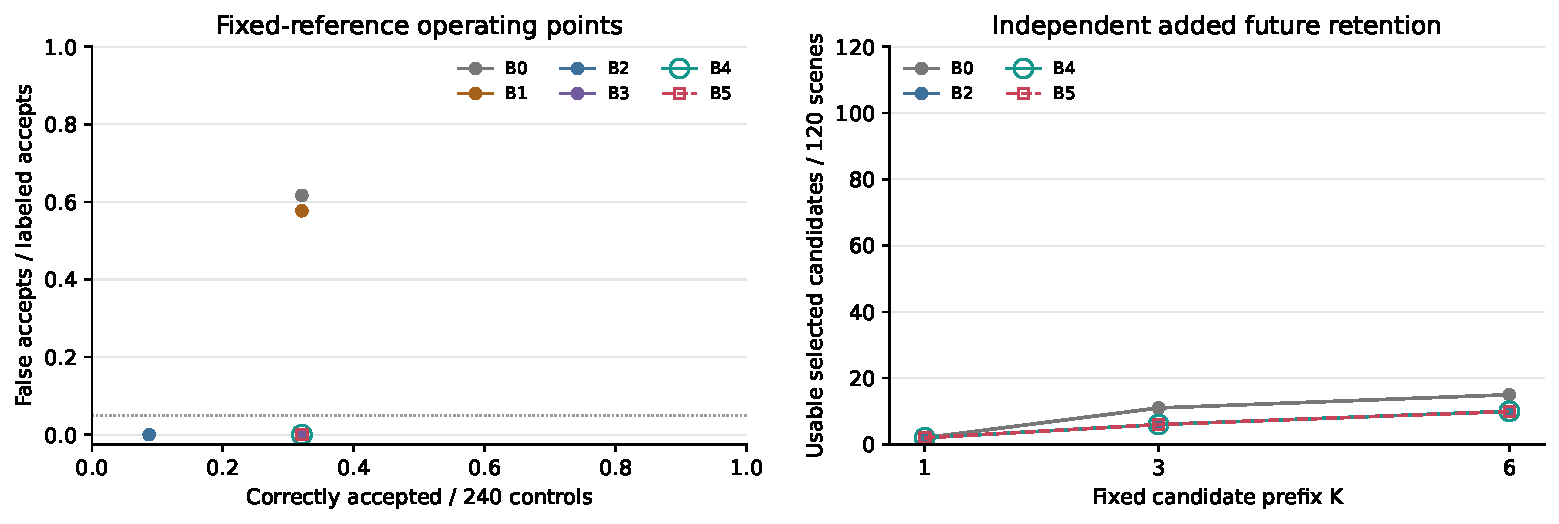
\includegraphics[width=\linewidth]{risk_coverage_utility.pdf}
\caption{Registered control operating points and sealed candidate decisions.
Curve points change both normalized force and torque bounds together relative
to the fixed nominal reference. Overlapping B4/B5 curves must not be interpreted
as independent performance gains. The utility panel reports all-scene counts.}
\label{fig:curves}
\end{figure}

\FloatBarrier

\section{Detailed Controls, References and Uncertainty}
\begin{table}[h]\centering\small\caption{Final control pass counts by registered apparatus group.}\label{tab:mechanisms}\begin{tabular}{lrrrrrr}\toprule
Group & N & B0 & B1 & B2 & B4 & B5\\\midrule
applied assistance & 30 & 0 & 0 & 0 & 0 & 0\\
boundary gap & 30 & 30 & 30 & 0 & 26 & 26\\
inactive margin & 30 & 30 & 30 & 0 & 30 & 30\\
independent & 30 & 21 & 21 & 21 & 21 & 21\\
intermittent floor & 30 & 30 & 11 & 0 & 0 & 0\\
necessary floor & 30 & 30 & 30 & 0 & 0 & 0\\
opposing environment & 30 & 30 & 30 & 0 & 0 & 0\\
redundant floor & 30 & 30 & 30 & 0 & 0 & 0\\
\bottomrule\end{tabular}\end{table}
\begin{table}[h]\centering\small\caption{Fixed counterfactual subsets; unreachable/invalid states are not replaced.}\label{tab:cf}\begin{tabular}{lrrrrrr}\toprule
Source & Both retain & Dependent & Rescue & Both fail & Unreached & Invalid\\\midrule
Controls & 33 & 6 & 0 & 0 & 9 & 0\\
Allegro & 0 & 1 & 0 & 0 & 19 & 0\\
Fetch & 7 & 0 & 0 & 0 & 13 & 0\\
Shadow/dgb & 16 & 0 & 0 & 0 & 4 & 0\\
\bottomrule\end{tabular}\end{table}

\begin{table}[h]\centering\small\caption{Mechanical baselines on the preselected branch subset. Valid and feasible/robust are separate counts; no-load truth is not their prediction target.}
\begin{tabular}{lrrrrr}\toprule
Source & Selected & B6 valid & B6 feasible & B7 valid & B7 robust\\\midrule
controls & 48 & 39 & 39 & 39 & 33\\
allegro & 20 & 0 & 0 & 1 & 0\\
fetch & 20 & 0 & 0 & 7 & 7\\
dexgraspbench & 20 & 0 & 0 & 16 & 14\\
\bottomrule\end{tabular}
\end{table}
\begin{table}[h]\centering\small\caption{Reference-sample labels and invalid telemetry. Allegro validity counts use 720 candidate executions, not independent scenes.}
\begin{tabular}{lrrrrrr}\toprule
Source & Executions & Invalid & Ref N & Ref P & Ref F & Ref U\\\midrule
controls & 240 & 0 & 240 & 77 & 163 & 0\\
allegro & 720 & 5 & 30 & 2 & 28 & 0\\
fetch & 100 & 0 & 30 & 0 & 15 & 15\\
dexgraspbench & 100 & 1 & 30 & 21 & 9 & 0\\
\bottomrule\end{tabular}
\end{table}
The full confusion matrices, FPR/FNR, conditional error rates, accepted risk, unknown bounds and source-specific denominators are in the machine-readable analysis. For example, no acceptance means accepted risk is NA, not zero; a reference-indeterminate accepted item contributes uncertainty rather than a verified true positive. Binomial Wilson intervals are explicitly conditional-iid summaries, not corrections for shared apparatus or few object identities. The raw reconstruction is code-independent, not simulator-independent.
Invalid Allegro candidate IDs from the geometry-consistency recovery are: \texttt{2ddbe9ae96604e624158}, \texttt{2658117c8f62d0ddfac4}, \texttt{c1963347598f1be128f4}, \texttt{555739848b81d855e167}, \texttt{a5eb27b988aecedb0b73}.

\FloatBarrier

\section{Historical Evidence and Candidate Library}
The earlier reports~\citep{teo_custom,teo_open} provide development provenance,
not new confirmation of this paper's monitor comparisons. Their reused
experimental history remains identifiable. The subsequent consolidated V3
experiment and present V4 study use different scene sets and analysis locks.
The earlier in-house hand study's 150/150 successes used an explicit assistance
mechanism and are not strict no-stabilizer successes; the locked final strict
evaluation was 0/150. Earlier open-hand validation reached 60/60 on the declared
three-family suites, whereas later frozen blind suites yielded 38/120 and
50/120 for the successive program versions. Those historical splits and
physical settings are not replaced or pooled with the present experiment.

In the preserved V3 compiled-primitive experiment, K6 native, contiguous and
environment-clear counts were 128,
122, and 37
for baseline, versus 141,
133, and 48
for repair, each over 360 scenes. The 11 clear-support gains were spheres.
Its actual uncertainty calculation was a paired scene bootstrap within six
fixed family strata of 60 scenes, 5,000 draws, seed 2026093040, two-sided 95\%
percentile interval: 1.67--4.72 percentage points. Candidates and blocks
were not separately resampled as independent scenes. All paired case keys
were required to exist; no missing-record imputation was used. This historical
analysis differs from the new registered 10,000-draw protocol.

On the same earlier 120 scenes, compiled primitive physics reduced no-contact
success from 18 to 13 for baseline and 24 to 18 for repair. This changes
geometry-dependent bounds and derived quantities as well as inertia, so it is
not an isolated inertia intervention. Repair native totals remained
43 versus 43 while 7 cases gained and
7 lost success. Equal totals therefore did not mean case-level
stability. A stricter definition is likewise not automatically more accurate
for a different target.

The present development retrospective covers 85 excluded
scenes and 510 candidate slots. Exactly
177 candidates were fully replayed with wrench telemetry;
333 already failed unchanged common
conditions. The new contract rescues 0/85
scenes. The 333 unmeasured load histories are not claimed to have zero load or
to have independent wrench-reference labels.

\begin{table}[h]\centering\small
\caption{Candidate membership in the historical V3 360-scene pool. Shared/new/dropped refer to distinct complete candidate specifications by family, not new independent program checkpoints.}
\begin{tabular}{lrrrrl}\toprule Family & Changed scenes & Shared & New & Dropped & Order / runner\\\midrule
bar & 0/60 & 11 & 0 & 0 & nearest XY / hold \\
capsule & 0/60 & 12 & 0 & 0 & nearest XY / hold \\
cube & 0/60 & 6 & 0 & 0 & fixed / staged \\
cylinder & 0/60 & 12 & 0 & 0 & nearest XY / hold \\
flat box & 0/60 & 6 & 0 & 0 & fixed / staged \\
sphere & 46/60 & 12 & 6 & 0 & nearest XY / hold \\
\bottomrule\end{tabular}\end{table}
The pool uses six candidates per scene; K=1 and K=3 are prefixes. There are no repeated candidates within a scene/policy prefix. No-extra equals baseline in all 360 scenes, rather than padding its budget with duplicates. The three conditions have 6,480 logical slots and share 2,278 distinct executions. Baseline has 29 complete candidate specifications and repair 35. Non-sphere ordered lists are unchanged; sphere additions alter the nearest-anchor neighborhood.
Candidate identity contains runner, anchor, derived-control offsets, hold extension and native thresholds. Staged schedules have pre-position, finger ramp/hold, thumb ramp/hold, lift and support phases. Hold schedules retain each anchor\textquotesingle s settling/contact/grip stages and any micro, bridge, cradle or feedback phases, followed by lift, support ramp and hold. Full numerical phase/control arrays are preserved in hash-locked anchor JSONs; no phase is refitted for V4.

\begin{table}[h]\centering\small
\caption{Realized geometry and mass ranges in the actual new V3 360 and V4 120 scene manifests, not substituted from an older 20-case suite. Box sizes are half-extents; curved objects use radius and axial half-length. All lengths below are mm and masses g.}
\begin{tabular}{llrrrrr}\toprule Split & Family & N & Size 1 & Size 2 & Size 3 & Mass\\\midrule
V3 & bar & 60 & 14.01--19.00 & 35.02--48.65 & 16.01--21.92 & 76.02--84.19 \\
V3 & capsule & 60 & 13.71--18.29 & 23.19--37.91 & 0.00--0.00 & 60.49--66.73 \\
V3 & cube & 60 & 22.01--28.23 & 22.01--28.23 & 22.01--28.23 & 55.01--64.35 \\
V3 & cylinder & 60 & 18.07--23.44 & 27.01--36.98 & 0.00--0.00 & 65.08--69.88 \\
V3 & flat box & 60 & 24.09--33.92 & 24.51--33.95 & 8.11--13.90 & 63.72--85.50 \\
V3 & sphere & 60 & 17.04--23.95 & 0.00--0.00 & 0.00--0.00 & 51.93--56.77 \\
V4 & bar & 20 & 14.37--18.80 & 35.54--48.68 & 16.01--21.83 & 76.32--84.21 \\
V4 & capsule & 20 & 13.62--18.43 & 23.13--37.05 & 0.00--0.00 & 61.02--66.19 \\
V4 & cube & 20 & 22.20--28.39 & 22.20--28.39 & 22.20--28.39 & 55.30--64.58 \\
V4 & cylinder & 20 & 18.03--23.38 & 27.88--36.50 & 0.00--0.00 & 65.63--68.78 \\
V4 & flat box & 20 & 24.03--33.95 & 24.20--33.07 & 8.19--13.81 & 65.25--84.11 \\
V4 & sphere & 20 & 17.19--23.97 & 0.00--0.00 & 0.00--0.00 & 52.03--56.78 \\
\bottomrule\end{tabular}\end{table}
The two studies use the same parametric family generator with different frozen seeds. V3 seeds are 2026093031--2026093033; V4 uses 2026100202 and records input-selection randomness before scene generation. Sizes and XY positions are drawn uniformly within family-specific ranges, but mass is a deterministic function of sampled size and height is coupled to the geometry: the lowest point starts 20 mm above the floor. Thus these are not independent mass/size/height factors or unseen object categories. Bar XY ranges are $[-2.5,8.5]\times[77,84.5]$ mm; other families use $[-9.5,9.5]\times[75,98.5]$ mm. Yaw is uniform within $\pm0.25$ rad for cubes, $\pm0.18$ for bars and $\pm0.30$ for flat boxes; rotationally symmetric families have zero initial yaw. Contact friction parameters remain $(0.9,0.015,0.004)$.
For the free-object apparatus, mass is uniform 50--100 g; half-extents are 25--35, 22--29 and 25--35 mm; pad friction is 0.55--0.90. Nominal jaw command is 10--16 mm, with nine deliberately weak hand-only initializations at 3.02--3.15 mm and necessary-floor command fixed at 3.1 mm. Inactive-floor gap is 10--14 mm and the boundary group uses 0.7 times that gap. Every third initialization uses either a lateral offset within $\pm7$ mm or tilt within $\pm0.15$ rad and angular speed within $\pm1$ rad/s. All values and their coupling are listed in the frozen input design.

\FloatBarrier

\subsection{Preserved V3 Comparisons}
The following original tables and figures retain V3's outcome definitions,
model pair and candidate budgets. Environment-clear means that study's
literal no-contact gate; it is not retrospectively renamed no-external-load.
\begin{table}[H]\centering\small
\caption{Same 120 scenes and frozen candidates: legacy runtime geometry edits versus per-case compiled primitive physics. Counts are coverage at $K=6$. Gains/losses compare physical conditions, not repaired versus baseline policies.}
\label{tab:v3-physics}
\begin{tabular}{llrrrr}\toprule
Program & Metric & Legacy & Compiled & Gains & Losses \\\midrule
baseline & Accumulated & 37 & 38 & 7 & 6 \\
baseline & Contiguous & 37 & 37 & 6 & 6 \\
baseline & Clear contiguous & 18 & 13 & 0 & 5 \\
repair & Accumulated & 43 & 43 & 7 & 7 \\
repair & Contiguous & 43 & 42 & 6 & 7 \\
repair & Clear contiguous & 24 & 18 & 0 & 6 \\
no-extra & Accumulated & 37 & 38 & 7 & 6 \\
no-extra & Contiguous & 37 & 37 & 6 & 6 \\
no-extra & Clear contiguous & 18 & 13 & 0 & 5 \\
\bottomrule\end{tabular}\end{table}

\begin{table}[H]\centering\small
\caption{Three new, fixed-size test blocks under compiled primitive physics. Each family contains 60 scenes; all rows use $K=6$. B: baseline; R: repair. Acc., cont., clear: original accumulated, contiguous, and environment-clear contiguous gates.}
\label{tab:v3-families}
\begin{tabular}{lrrrrrr}\toprule
Family & Acc. B & Acc. R & Cont. B & Cont. R & Clear B & Clear R \\\midrule
Cube & 49 & 49 & 49 & 49 & 0 & 0 \\
Cylinder & 35 & 35 & 34 & 34 & 34 & 34 \\
Bar & 21 & 21 & 21 & 21 & 0 & 0 \\
Sphere & 2 & 15 & 2 & 13 & 2 & 13 \\
Capsule & 1 & 1 & 1 & 1 & 1 & 1 \\
Flat box & 20 & 20 & 15 & 15 & 0 & 0 \\
Total / 360 & 128 & 141 & 122 & 133 & 37 & 48 \\
\bottomrule\end{tabular}\end{table}

\begin{table}[H]\centering\small
\caption{Fixed candidate prefixes on all 360 new scenes. Selected-clear scores the unchanged original outcome-aware selector; clear coverage is the existence of a passing candidate under the corrected contract.}
\label{tab:v3-budget}
\begin{tabular}{lrrrrr}\toprule
Program & $K$ & Accumulated & Contiguous & Clear coverage & Selected-clear \\\midrule
baseline & 1 & 48 & 46 & 11 & 11 \\
baseline & 3 & 111 & 106 & 27 & 27 \\
baseline & 6 & 128 & 122 & 37 & 37 \\
repair & 1 & 52 & 49 & 14 & 14 \\
repair & 3 & 122 & 115 & 36 & 36 \\
repair & 6 & 141 & 133 & 48 & 48 \\
\bottomrule\end{tabular}\end{table}

\begin{table}[H]\centering\small
\caption{Replication and anchor-removal ablation under the clear-contiguous contract ($K=6$). Each new block was fixed at 120 scenes before execution. Gains/losses are paired program differences within each block.}
\label{tab:v3-blocks}
\begin{tabular}{lrrrrrr}\toprule
Block & $N$ & Baseline & Repair & No extra & Gains & Losses \\\midrule
Block 1 & 120 & 11 & 15 & 11 & 4 & 0 \\
Block 2 & 120 & 13 & 17 & 13 & 4 & 0 \\
Block 3 & 120 & 13 & 16 & 13 & 3 & 0 \\
Combined & 360 & 37 & 48 & 37 & 11 & 0 \\
\bottomrule\end{tabular}\end{table}

\begin{figure}[H]
\centering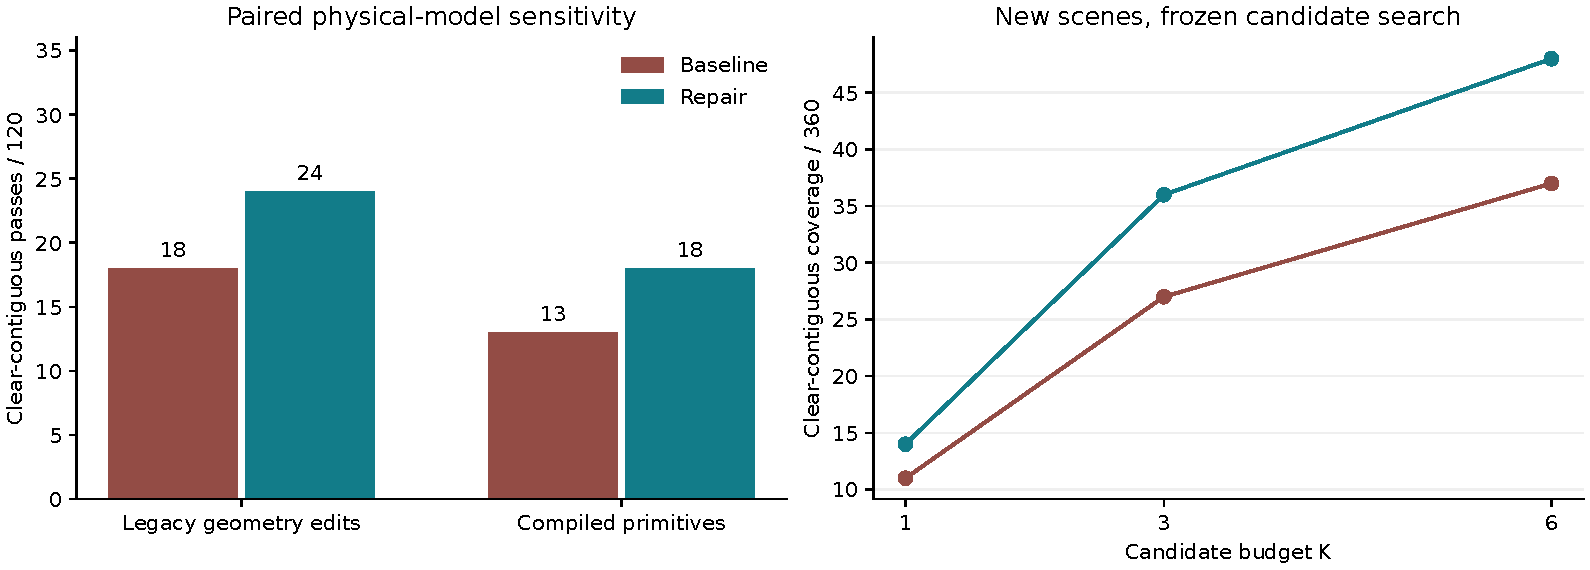
\includegraphics[width=.94\linewidth]{v3_physics_and_budget.pdf}
\caption{Preserved V3 model and budget comparison. Model changes were not an
isolated inertia intervention. Historical intervals and denominators differ
from V4 and are not pooled with it.}
\end{figure}
\begin{figure}[H]
\centering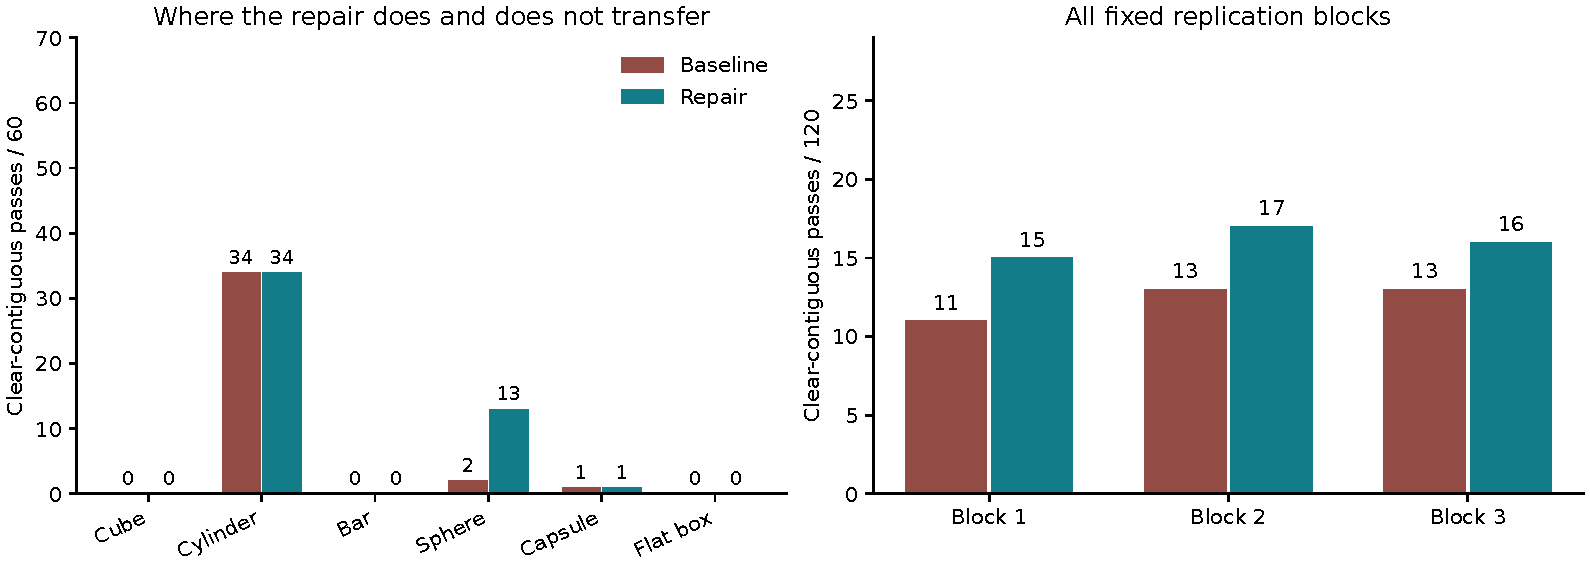
\includegraphics[width=.94\linewidth]{v3_family_replication.pdf}
\caption{Preserved V3 family-level results. The 11 no-contact gains occur in
spheres; this does not establish broad family generalization.}
\end{figure}

\section{Numerical Qualification and Recovery}
The observer reads each physical contact solve without inserting a forward
solve into the live trajectory. Target-directed wrenches use the geom-2
convention of \texttt{mj\_contactForce}. Contact geometry/forces belong to the
pre-integration solve state; post-integration poses and velocities have
separate fields. Integer step indices and measured timestamps are retained
without decimation for adjudication. Full snapshots include warm starts,
controls, applied forces and mocap; both branches consume the same input tape.
The branch gate uses prefix conditions and local $Q$, not future native success.

The 80 calibration controls contain 25 no-load reference passes and 55 failures;
B4/B5 match all 80. Development branches have 57 both-retain, 10 dependent and
13 unreachable states. Thirty-two executions of the first eight controls vary
timestep and solver iterations; they are repeated numerical conditions, not
32 new scenes. A selected natural 20-scene development subset has 17 dependent
and three both-retain late states, with pre-branch load in the latter. All
20 labels remain unchanged under the registered numerical settings. These
selected exclusions do not estimate natural prevalence. A simple pre-branch
load threshold separates that subset, so no superior learned dependency
predictor is introduced. Four additional single-burst development cases show
16.9\,s accumulated versus 9.9\,s continuous unloaded $Q$; they are not added
to the 80-case calibration denominator.

The five Allegro geometry failures were retained using a post-failure,
fail-closed bookkeeping recovery. Its hash is separate from the input-only
protocol lock. No threshold, physical parameter, candidate, data role or
primary comparison was changed. Invalid telemetry and physical indeterminacy
are separate fields that can overlap; neither may be silently recoded as a
verified failure. Natural references were simple random samples (30/120
rank-1 Allegro entries; 30/100 for Fetch and DGB), not selected successes.

\section{Offline Reproduction and Raw-Evidence Scope}
The label evidence archive contains execution scores, reference labels,
all 720 candidate future endpoints, the pre-future choice seal, protocol and
source manifests, operating-point labels, code, recovery provenance and claim
ledger. Its protocol SHA256 remains
\path{ffc60fe94dca45e826c2f864865cbeb7c749b7a11b6f05784b9c6f24b896b9a0}.
The frozen scientific files are unchanged; V4.5 adds only manuscript,
figure-composition and packaging files.

Extract the label evidence archive. From its top-level directory, run:
\begin{lstlisting}
python -B reproduce_v4/reproduce.py --out ../v4-recomputed
\end{lstlisting}
Use a new output directory. Python 3.11, NumPy and Matplotlib are required.
The original verifier blocks MuJoCo imports and network connections, verifies
packaged hashes before and after computation, recomputes source tables and
paired intervals from individual labels, reconstructs U2 from sealed choices
and future endpoints, and checks operating curves and the claim ledger. It
also reconstructs the three original V4 figures and rescores three included
primitive-control raw examples. It does not replay physics.

The V4.5 publication-only figure command is separate:
\begin{lstlisting}
python -B scripts/v45_editorial.py figures
\end{lstlisting}
It uses the same recorded JSON/CSV and saved display arrays, checks the
displayed counts, and composes the three main-paper figures. The four-cell
example table comes from recorded control outcomes, not a new simulation.
The selection stacks classify failures only after checking the corresponding
future status is valid; unclassified returned outcomes cause an error.

\paragraph{What is supplied.}
The label package includes all individual scored records needed for the
reported aggregates. The separate core-raw ZIP includes all 240 nominal final
primitive-control NPZs and their eight margin/gap partners, with a dedicated
hash/size manifest. These controls contain original primitive apparatus
models, not redistributed third-party hand meshes. The companion is optional
for label-level reproduction; it is additional source evidence, not a claim
that all 248 raw records have been independently re-adjudicated during this
editorial release. The original verifier's three raw rescoring examples remain
the verified raw-reconstruction scope.

\paragraph{What is not supplied or claimed.}
Most natural-task, calibration and retrospective raw NPZs remain in the local
archive. The full raw inventory records hashes and sizes, but an inventory is
not raw access. No public host for the complete archive is asserted. Thus
aggregate reproduction, access to controlled raw evidence, full-matrix raw
adjudication, and dynamic reproduction are distinct levels. No complete
independent raw audit or clean-machine simulation rerun is claimed.

Main experiments used CPython 3.11.1, NumPy 2.4.6, MuJoCo 3.8.0 and SciPy
1.17.1; DGB used NumPy 1.26.4 and MuJoCo 3.3.2. Offline release checks used
NumPy 1.26.4 and Matplotlib 3.11.2. The preserved first-case dynamic checks
cover all four sources in existing isolated environments; they are not
fresh installations or complete-matrix reruns. V4.5 adds no dynamic check.

\paragraph{External provenance.}
FetchExpert~\citep{fetch_expert} is pinned to commit
\path{3e2dd8c2e5f24702081867d82a78eb1264534f94}, file
\path{experts/fetch_expert.py}; Gymnasium-Robotics~\citep{gymnasium_robotics}
is version 1.4.2 (FetchPickAndPlace-v4). DGB is pinned to
\path{d9ea6cf282de1f463c20fa54b4f68d7025bad40e}. Dependency records list
component-specific licenses and hashes. Third-party model assets and the
unlicensed DGB checkout are excluded; missing assets are not silently
downloaded, substituted or reported as dynamically verified. No new license
grant for the author's source is made by this local package.

\section{Disclosure}
OpenAI Codex assisted implementation, experimental workflow, analysis tooling,
figure composition and manuscript preparation under author direction. The
author is responsible for all claims and the final submission. No controlled
comparison estimates the assistance's causal effect.

\FloatBarrier
\begingroup
\small
\setlength{\bibsep}{2pt}
\bibliographystyle{plainnat}
\bibliography{references,provenance}
\endgroup
\end{document}
